% -----------------------------------------------------------------------------
% Narrativa principal: 12 slides, 18 min 15 s.
% -----------------------------------------------------------------------------

% Slide 1 ---------------------------------------------------------------------
\begin{frame}
  \slidetime{0:45}
  \vspace{0.14cm}
  \eyebrow{CoInfoSim \enspace\textbullet\enspace apresentação acadêmica}

  \vspace{0.22cm}
  \begin{columns}[c,onlytextwidth]
    \begin{column}{0.71\textwidth}
      {\bfseries\fontsize{19.5}{23.5}\selectfont\color{CoInfoInk}
        Preservação da estrutura\\de cooperação entre\\canais de informação\par}

      \vspace{0.26cm}
      {\fontsize{11.6}{14.6}\selectfont\color{CoInfoBlue}
        O treinamento com amostras sintéticas reproduz a\\evolução da cooperação observada com amostras reais?\par}

      \vspace{0.32cm}
      {\fontsize{9.4}{11.6}\selectfont
        \textbf{Paulo Renato Azevedo}\par
        Programa de Pós-Graduação em Informática \textbullet{} UFRJ\par
        \textcolor{CoInfoGray}{Ciência de Dados \textbullet{} 2026}}
    \end{column}
    \begin{column}{0.26\textwidth}
      \centering
      \begin{tikzpicture}[x=0.74cm,y=0.74cm]
        \foreach \x/\y/\r in {0/2.8/0.25,1.5/3.5/0.22,2.9/2.7/0.24,0.6/1.3/0.23,2.3/1.2/0.26,1.5/0/0.28}{
          \fill[CoInfoPale] (\x,\y) circle (\r+0.12);
          \draw[CoInfoBlue!75,line width=1.0pt] (\x,\y) circle (\r);
        }
        \draw[CoInfoLavender!80,line width=0.9pt] (0.2,2.65)--(1.28,3.35)--(2.65,2.77)--(2.25,1.45)--(1.55,0.25)--(0.75,1.45)--cycle;
        \draw[CoInfoAmber,line width=1.4pt] (0.25,2.65) .. controls (1.0,2.2) and (1.75,2.2) .. (2.65,2.67);
        \node[font=\bfseries\fontsize{8.6}{10.2}\selectfont,text=CoInfoInk] at (1.48,-0.85) {subconjuntos de canais};
        \node[font=\fontsize{7.6}{9.0}\selectfont,text=CoInfoGray,align=center] at (1.48,-1.50) {desempenho relativo que\\muda com o tamanho amostral};
      \end{tikzpicture}
    \end{column}
  \end{columns}

  \vspace{0.30cm}
  \takeaway{Amostras sintéticas não são usadas para aumentar a acurácia: investigamos se o treinamento sintético reproduz a cooperação observada com o treinamento real.}

  \speakernotes
    {Neste trabalho, as amostras sintéticas não são usadas para aumentar a acurácia do classificador. Elas são usadas para investigar se o treinamento sintético reproduz o comportamento cooperativo dos subconjuntos de canais observado com treinamento real. O objeto de interesse é comparativo: treinamos os mesmos classificadores com amostras reais ou sintéticas, avaliamos no mesmo teste real fixo e observamos se o desempenho relativo dos subconjuntos evolui da mesma forma. Essa estrutura só aparece depois do treinamento e da avaliação dos classificadores; ela não está pronta dentro das amostras nem pertence ao modelo gerador. A pergunta é simples, mas exigente: ao trocar a origem das amostras de treinamento, preservamos quem tende a cooperar com quem e em quais regimes amostrais?}
    {Para entender por que essa pergunta importa, começo pela decisão operacional que existe antes de qualquer gerador sintético.}
    {O estudo avalia a reprodução do comportamento cooperativo, não o aumento de acurácia.}
    {45 segundos.}
    {Não atribuir a estrutura às amostras sintéticas ou ao gerador; ela emerge das perdas após o treinamento e a avaliação dos classificadores.}
\end{frame}

% Slide 2 ---------------------------------------------------------------------
\begin{frame}{Por que comparar subconjuntos de canais?}
  \slidetime{1:20}
  \vspace{-0.06cm}
  \centering
  \begin{tikzpicture}[x=1cm,y=0.86cm,
    source/.style={rounded corners=3pt,draw=CoInfoBlue!40,fill=CoInfoPale,
      minimum width=3.30cm,minimum height=0.96cm,align=center,
      font=\fontsize{9.4}{11.2}\selectfont,text=CoInfoInk},
    channel/.style={rounded corners=2pt,draw=CoInfoBlue!70,fill=white,
      minimum width=0.72cm,minimum height=0.55cm,font=\bfseries\small,text=CoInfoInk},
    target/.style={rounded corners=3pt,fill=CoInfoBlue,
      text=white,minimum width=4.55cm,minimum height=0.82cm,align=center,
      font=\bfseries\fontsize{9.8}{11.8}\selectfont}]
    \node[source] (s1) at (1.85,4.50) {Sensores ambientais\\temperatura, CO$_2$, luz};
    \node[source] (s2) at (6.35,4.50) {Medições fisiológicas\\ou laboratoriais};
    \node[source] (s3) at (10.85,4.50) {Equipamentos, sistemas\\ou especialistas};

    \node[channel] (x1) at (3.55,2.95) {$X_1$};
    \node[channel] (x2) at (4.55,2.95) {$X_2$};
    \node[channel] (x3) at (5.55,2.95) {$X_3$};
    \node[font=\large,text=CoInfoGray] at (6.40,2.95) {$\cdots$};
    \node[channel] (xd) at (7.25,2.95) {$X_d$};
    \node[font=\fontsize{8.5}{10}\selectfont,text=CoInfoGray] at (9.05,2.95) {canais disponíveis};

    \node[target] (target) at (5.40,1.52) {um classificador para cada subconjunto};
    \draw[-{Stealth[length=2.3mm]},CoInfoBlue!55,line width=.8pt] (s1.south) -- (x1.north);
    \draw[-{Stealth[length=2.3mm]},CoInfoBlue!55,line width=.8pt] (s2.south) -- (x3.north);
    \draw[-{Stealth[length=2.3mm]},CoInfoBlue!55,line width=.8pt] (s3.south) -- (xd.north);
    \draw[-{Stealth[length=2.3mm]},CoInfoBlue,line width=.95pt] (5.40,2.60) -- (target.north);

    \foreach \x/\txt/\cname in {1.85/informação/CoInfoMint,4.85/redundância/CoInfoBlue,7.85/complexidade/CoInfoAmber,10.85/custo operacional/CoInfoRose}{
      \node[rounded corners=8pt,draw=\cname!55,fill=\cname!7,
        font=\bfseries\fontsize{8.6}{10}\selectfont,text=CoInfoInk,
        minimum width=2.45cm,minimum height=.52cm] at (\x,0.30) {\txt};
    }
  \end{tikzpicture}

  \vspace{0.14cm}
  \takeaway{Antes de decidir quais canais manter, remover ou combinar, é necessário compreender como eles cooperam na classificação.}
  \sourcecite{Guyon e Elisseeff (2003); Brown et al. (2012); Hughes (1968); Raudys e Jain (1991).}

  \speakernotes
    {Em operações reais, cada variável pode representar um sensor ambiental, um exame, uma medição fisiológica, uma saída de equipamento ou informação produzida por um especialista. Adicionar canais pode trazer sinal complementar, mas também redundância, maior dimensionalidade, complexidade de integração e custo operacional. Com poucas amostras, acrescentar dimensões pode inclusive aumentar a dificuldade de estimação, o conhecido efeito de pequenas amostras associado ao fenômeno de Hughes. O trabalho não resolve a decisão econômica. Ele constrói uma etapa anterior: mapear como todos os subconjuntos de canais se comportam na tarefa de classificação, treinando um classificador para cada subconjunto. Se a estrutura resultante puder ser reproduzida pelo treinamento com amostras sintéticas, teremos informação estrutural para estudos operacionais posteriores.}
    {A motivação operacional leva à definição precisa do que chamo de estrutura de cooperação.}
    {Compreender a cooperação vem antes de escolher, retirar ou precificar canais.}
    {1 minuto e 20 segundos.}
    {Custo aparece apenas como motivação e camada futura; este experimento não otimiza custos nem demonstra economia.}
\end{frame}

% Slide 3 ---------------------------------------------------------------------
\begin{frame}{O que é a estrutura de cooperação?}
  \slidetime{2:00}
  \centering
  \begin{tikzpicture}[x=1.02cm,y=0.42cm]
    \fill[CoInfoPale!60] (0.65,0.6) rectangle (3.0,5.42);
    \fill[CoInfoMist] (3.0,0.6) rectangle (5.45,5.42);
    \fill[CoInfoCream!75] (5.45,0.6) rectangle (8.15,5.42);
    \draw[-{Stealth[length=2.3mm]},CoInfoGray,line width=.8pt] (0.65,0.6)--(8.38,0.6);
    \draw[-{Stealth[length=2.3mm]},CoInfoGray,line width=.8pt] (0.65,0.6)--(0.65,5.60);
    \node[rotate=90,align=center,font=\fontsize{7.8}{9.0}\selectfont,text=CoInfoGray] at (0.30,3.05) {perda média\\no teste real};
    \node[font=\fontsize{8.2}{9.8}\selectfont,text=CoInfoGray] at (4.55,-0.14) {amostras de treinamento por classe, $n$};
    \node[font=\scriptsize,text=CoInfoGray] at (1.80,5.05) {poucas amostras};
    \node[font=\scriptsize,text=CoInfoGray] at (4.20,5.05) {transição};
    \node[font=\scriptsize,text=CoInfoGray] at (6.77,5.05) {mais amostras};

    \draw[CoInfoBlue,line width=1.7pt]
      plot[smooth] coordinates {(0.80,2.00) (1.7,1.75) (2.8,1.58) (4.1,1.50) (5.5,1.46) (7.9,1.43)};
    \draw[CoInfoAmber,line width=1.7pt]
      plot[smooth] coordinates {(0.80,4.45) (1.7,3.25) (2.8,2.05) (4.1,1.42) (5.5,1.05) (7.9,0.90)};
    \draw[CoInfoPlum,line width=1.7pt]
      plot[smooth] coordinates {(0.80,5.00) (1.7,4.10) (2.8,3.10) (4.1,2.05) (5.5,1.18) (7.9,0.67)};

    \fill[CoInfoAmber] (3.78,1.50) circle (1.9pt);
    \fill[CoInfoPlum] (5.25,1.25) circle (1.9pt);
    \draw[dashed,CoInfoAmber!75] (3.78,0.60)--(3.78,1.50);
    \draw[dashed,CoInfoPlum!75] (5.25,0.60)--(5.25,1.25);

    \node[anchor=west,font=\bfseries\fontsize{7.4}{8.8}\selectfont,text=CoInfoBlue] at (8.24,1.60) {$\{X_1\}$};
    \node[anchor=west,font=\bfseries\fontsize{7.4}{8.8}\selectfont,text=CoInfoAmber] at (8.24,1.02) {$\{X_1,X_3\}$};
    \node[anchor=west,font=\bfseries\fontsize{7.4}{8.8}\selectfont,text=CoInfoPlum] at (8.24,0.44) {$\{X_1,X_2,X_3\}$};
  \end{tikzpicture}

  \vspace{0.06cm}
  \begin{columns}[T,onlytextwidth]
    \begin{column}{0.32\textwidth}
      \infocard{1. Desempenho}{para cada subconjunto, um classificador é treinado e avaliado}
    \end{column}
    \begin{column}{0.32\textwidth}
      \infocard{2. Ranking em cada $n$}{subconjuntos ordenados pela perda média no teste real}
    \end{column}
    \begin{column}{0.32\textwidth}
      \infocard{3. Evolução com $n$}{o desempenho relativo muda quando $n$ cresce}
    \end{column}
  \end{columns}

  \vspace{0.06cm}
  \takeaway{A estrutura de cooperação descreve como o desempenho relativo dos subconjuntos de canais evolui à medida que o tamanho do conjunto de treinamento aumenta.}
  \sourcecite{elaboração própria; esquema conceitual, sem valores experimentais.}

  \speakernotes
    {A estrutura começa com curvas de perda no mesmo teste real. Para cada tamanho de treinamento por classe, cada subconjunto origina um classificador e uma perda média estimada por Monte Carlo. Para cada tamanho amostral, os subconjuntos são então ordenados por seu desempenho preditivo, medido pela perda média no teste real. Com poucas amostras, um canal isolado pode ter menor perda porque exige menos estimação; à medida que o treinamento cresce, um par ou um conjunto maior pode aproveitar informação complementar e ultrapassá-lo. A hierarquia tem três degraus: o desempenho preditivo pertence a cada subconjunto; o ranking de desempenho compara os subconjuntos em um dado $n$; e a estrutura de cooperação é a evolução dessas posições relativas quando $n$ cresce. Portanto, cooperação não é correlação bruta entre variáveis nem uma propriedade inscrita nas amostras: é uma organização dinâmica produzida pelo treinamento dos classificadores e pela comparação de suas perdas ao longo da grade amostral.}
    {Com o objeto definido, posso formular a pergunta científica sem confundi-la com aumento de dados ou melhoria preditiva.}
    {A estrutura não é um ranking estático: é a evolução do desempenho relativo ao longo de $n$.}
    {2 minutos.}
    {O gráfico é conceitual, sem valores experimentais; não interpretar os cruzamentos desenhados como resultados de um dataset.}
\end{frame}

% Slide 4 ---------------------------------------------------------------------
\begin{frame}{Pergunta científica e escopo}
  \slidetime{1:20}
  \vspace{0.22cm}
  \begin{beamercolorbox}[wd=\linewidth,sep=0.34cm,rounded=true]{block body}
    \centering\bfseries\fontsize{14.6}{18.6}\selectfont\color{CoInfoInk}
    Em que medida a estrutura de cooperação que emerge do treinamento de classificadores com amostras sintéticas reproduz aquela que emerge do treinamento dos mesmos classificadores com amostras reais?
  \end{beamercolorbox}

  \vspace{0.54cm}
  \begin{columns}[onlytextwidth]
    \begin{column}{0.31\textwidth}
      \begin{beamercolorbox}[wd=\linewidth,ht=1.24cm,dp=.20cm,sep=.12cm,rounded=true]{block body}
        \centering\bfseries\fontsize{11.2}{13.6}\selectfont\color{CoInfoRose}
        Não é aumento\\de dados.
      \end{beamercolorbox}
    \end{column}
    \begin{column}{0.31\textwidth}
      \begin{beamercolorbox}[wd=\linewidth,ht=1.24cm,dp=.20cm,sep=.12cm,rounded=true]{block body}
        \centering\bfseries\fontsize{11.2}{13.6}\selectfont\color{CoInfoRose}
        Não é busca de\\maior acurácia.
      \end{beamercolorbox}
    \end{column}
    \begin{column}{0.31\textwidth}
      \begin{beamercolorbox}[wd=\linewidth,ht=1.24cm,dp=.20cm,sep=.12cm,rounded=true]{block body}
        \centering\bfseries\fontsize{11.2}{13.6}\selectfont\color{CoInfoMint}
        É avaliar a preservação da\\estrutura de cooperação.
      \end{beamercolorbox}
    \end{column}
  \end{columns}

  \vfill
  \sourcecite{estratégia inspirada em Train on Synthetic, Test on Real: Esteban, Hyland e Rätsch (2017).}

  \speakernotes
    {A comparação é entre duas estruturas emergentes. Na referência, os classificadores são treinados com amostras reais. Nos braços sintéticos, os mesmos classificadores são treinados com amostras produzidas por modelos geradores parametrizados a partir do reservatório real. Em todos os casos, a avaliação ocorre no mesmo teste real fixo. Esse desenho se aproxima da lógica Train on Synthetic, Test on Real, mas o desfecho principal não é a perda isolada: o que se compara é o padrão relativo entre todos os subconjuntos, isto é, a ordenação por perda média, as vitórias par a par e a dinâmica das transições. Por isso, uma condição sintética pode reproduzir a estrutura de cooperação sem produzir a menor perda absoluta, e o inverso também pode ocorrer.}
    {A pergunta exige um protocolo em que somente a origem das amostras de treinamento mude.}
    {O alvo é a preservação da estrutura de cooperação, não aumento de dados nem ganho de acurácia.}
    {1 minuto e 20 segundos.}
    {Não nomear os braços como se o modelo gerador treinasse o classificador; são classificadores treinados com amostras produzidas por esses modelos.}
\end{frame}

% Slide 5 ---------------------------------------------------------------------
\begin{frame}{Três braços, um único teste real}
  \slidetime{2:00}
  \centering
  \vspace{0.02cm}
  
\includegraphics[width=0.92\linewidth,height=4.78cm,keepaspectratio]{\figroot/conceptual/pipeline_condicoes.pdf}

  \vspace{0.10cm}
  \metricpill{CoInfoBlue}{Grade}{\(n=2,\ldots,512\) por classe}
  \hspace{0.04cm}
  \metricpill{CoInfoMint}{Monte Carlo}{replicações até precisão alvo}
  \hspace{0.04cm}
  \metricpill{CoInfoAmber}{Subconjuntos}{não vazios: 31 ou 127}

  \sourcecite{elaboração própria (figura do protocolo experimental, também usada no relatório final).}

  \speakernotes
    {O ponto de partida é um reservatório real de treinamento. A padronização e a parametrização dos modelos geradores usam somente esse reservatório. No primeiro braço, Real para Real, cada replicação sorteia amostras reais balanceadas por classe. No segundo, uma Gaussiana única por classe, parametrizada a partir dos dados reais de treinamento no espaço completo de canais, produz as amostras sintéticas. No terceiro, um GMM por classe é parametrizado a partir dos mesmos dados; o número de componentes é escolhido por BIC. Para cada tamanho da grade, repetimos o treinamento de cada classificador em todos os subconjuntos não vazios: 31 quando há cinco canais e 127 quando há sete. As replicações Monte Carlo estimam as perdas médias. A única coisa que muda entre os braços é a origem das amostras de treinamento. O conjunto de teste real é fixo e compartilhado; é ele que permite comparar, em uma base comum, as estruturas obtidas após o treinamento. No cenário full-scale do Air Quality, a mesma grade é estendida até 1024 amostras por classe.}
    {Das perdas médias desse protocolo derivam as três métricas, começando pela visão mais global.}
    {Real, Gaussiana única e GMM mudam a origem do treinamento; o teste real permanece exatamente o mesmo.}
    {2 minutos.}
    {``Gaussiana única \(\rightarrow\) Real'' e ``GMM \(\rightarrow\) Real'' significam treinamento com amostras sintéticas e teste no conjunto real fixo; a estrutura não pertence ao gerador.}
\end{frame}

% Slide 6 ---------------------------------------------------------------------
\begin{frame}{Métrica 1 — a ordenação global foi preservada?}
  \slidetime{1:20}
  \begin{columns}[T,onlytextwidth]
    \begin{column}{0.50\textwidth}
      \centering
      \vspace{0.10cm}
      
\includegraphics[height=3.92cm,trim=0 56 322 0,clip]{\figroot/conceptual/metricas_tres_paineis.pdf}
    \end{column}
    \begin{column}{0.47\textwidth}
      \vspace{0.12cm}
      \infocard{Cada $n$ produz uma ordenação completa}{por perda média, não só o primeiro colocado}
      \vspace{0.10cm}
      \infocard{Correlação de Spearman}{ordenação sintética vs.\ referência Real $\rightarrow$ Real}
      \vspace{0.10cm}
      \infocard{$\rankrho\approx1$}{organização global semelhante nos dois treinamentos}
    \end{column}
  \end{columns}

  \vspace{0.06cm}
  \takeaway{Correlação alta tolera trocas locais; não exige o mesmo primeiro colocado.}
  \sourcecite{figura conceitual do relatório final; Spearman (1904).}

  \speakernotes
    {Em cada tamanho amostral, ordenamos todos os subconjuntos pela perda média no teste real. A correlação de Spearman compara os vetores de postos do braço sintético com a referência Real para Real. É uma medida global: se dois subconjuntos quase empatados trocam de posição, a correlação pode continuar muito alta. Isso é importante porque a estrutura não deve ser reduzida ao primeiro colocado. No Occupancy, por exemplo, o braço treinado com amostras do GMM repetiu o vencedor do braço real no SVM, mas o braço da Gaussiana única produziu um ranking completo mais próximo da referência. Portanto, ``acertar o melhor'' e preservar a ordenação da lista inteira são afirmações diferentes.}
    {A ordenação global ainda pode esconder quais decisões específicas entre pares foram preservadas; a segunda métrica abre essa estrutura.}
    {Ranking de desempenho significa a lista inteira ordenada por perda média, não somente quem ficou em primeiro.}
    {1 minuto e 20 segundos.}
    {Correlação alta não implica igualdade das perdas nem identidade do topo; ela mede associação entre postos.}
\end{frame}

% Slide 7 ---------------------------------------------------------------------
\begin{frame}{Métrica 2 — decisões ``A vence B''}
  \slidetime{1:20}
  \begin{columns}[T,onlytextwidth]
    \begin{column}{0.51\textwidth}
      \centering
      \vspace{0.10cm}
      
\includegraphics[height=3.85cm,trim=156 52 156 0,clip]{\figroot/conceptual/metricas_tres_paineis.pdf}
    \end{column}
    \begin{column}{0.46\textwidth}
      \vspace{0.16cm}
      \infocard{Para cada par de subconjuntos}{vence o que obtém menor perda média; empates exatos são excluídos}
      \vspace{0.20cm}
      \infocard{\WA{}}{proporção de pares com o mesmo vencedor nos braços real e sintético}
      \vspace{0.20cm}
      \begin{tikzpicture}
        \node[rounded corners=3pt,draw=CoInfoMint!60,fill=CoInfoMint!7,
          font=\bfseries\fontsize{9.0}{10.7}\selectfont,text=CoInfoInk,inner sep=4.5pt]
          {uma troca no topo $\neq$ colapso da estrutura};
      \end{tikzpicture}
    \end{column}
  \end{columns}

  \vspace{0.12cm}
  \takeaway{Quantas relações de superioridade entre alternativas permanecem iguais?}
  \sourcecite{definição e figura conceitual do relatório final do CoInfoSim.}

  \speakernotes
    {Agora comparamos cada par de subconjuntos. Se a perda média de A é menor que a de B, registramos que A vence B. A Winners Agreement é a proporção dessas decisões que coincide entre o braço sintético e a referência real, excluindo empates exatos, que não têm vencedor estrito comparável. Para 31 subconjuntos existem 465 pares; para 127, 8.001. A métrica é operacionalmente intuitiva: mesmo que haja uma troca residual entre os dois primeiros lugares, centenas de relações entre alternativas podem permanecer idênticas. Ela informa quanto do mapa decisório foi conservado, não apenas quem ocupa a primeira linha.}
    {Ranking e vencedores observam um ponto da grade; a terceira métrica adiciona explicitamente a dinâmica do tamanho amostral.}
    {Winners Agreement mede a preservação das decisões par a par.}
    {1 minuto e 20 segundos.}
    {Não interpretar a matriz quadrada como pares duplicados na métrica; o cálculo usa cada par não ordenado uma única vez e exclui empates.}
\end{frame}

% Slide 8 ---------------------------------------------------------------------
\begin{frame}{Métrica 3 — quando a superioridade muda?}
  \slidetime{1:50}
  \begin{columns}[T,onlytextwidth]
    \begin{column}{0.56\textwidth}
      \centering
      \vspace{0.04cm}
      \begin{tikzpicture}[x=0.72cm,y=0.465cm]
        % regiões antes/depois do cruzamento
        \fill[CoInfoPale!60] (0.65,0.6) rectangle (6.0,5.30);
        \fill[CoInfoCream!75] (6.0,0.6) rectangle (9.55,5.30);
        \draw[-{Stealth[length=2.3mm]},CoInfoGray,line width=.8pt] (0.65,0.6)--(9.80,0.6);
        \draw[-{Stealth[length=2.3mm]},CoInfoGray,line width=.8pt] (0.65,0.6)--(0.65,5.50);
        \node[rotate=90,font=\fontsize{8.4}{10}\selectfont,text=CoInfoGray] at (0.10,3.0) {perda média no teste real};
        \node[font=\fontsize{8.4}{10}\selectfont,text=CoInfoGray] at (5.1,0.02) {amostras de treinamento por classe, $n$};

        % duas curvas suaves, decrescentes, com um único cruzamento
        \draw[CoInfoBlue,line width=1.9pt]
          plot[smooth] coordinates {(0.90,2.55) (2.2,2.18) (4.0,1.97) (6.0,1.85) (7.6,1.80) (9.1,1.77)};
        \draw[CoInfoAmber,line width=1.9pt]
          plot[smooth] coordinates {(0.90,4.85) (2.2,3.62) (4.0,2.62) (6.0,1.85) (7.6,1.42) (9.1,1.26)};

        % cruzamento único, marcado como N*
        \draw[dashed,CoInfoPlum,line width=0.9pt] (6.0,0.6)--(6.0,4.55);
        \fill[CoInfoPlum] (6.0,1.85) circle (2.3pt);
        \node[font=\bfseries\fontsize{10.5}{12}\selectfont,text=CoInfoPlum] at (6.0,4.95) {$N^{\star}$};

        % rótulos das curvas
        \node[anchor=west,font=\bfseries\scriptsize,text=CoInfoBlue] at (9.15,1.79) {$S_A$};
        \node[anchor=west,font=\bfseries\scriptsize,text=CoInfoAmber] at (9.15,1.24) {$S_B$};

        % anotações das regiões
        \node[font=\fontsize{8.2}{9.8}\selectfont,text=CoInfoInk,align=center] at (3.15,1.22)
          {Antes de $N^{\star}$:\\$S_A$ apresenta menor perda.};
        \node[font=\fontsize{8.2}{9.8}\selectfont,text=CoInfoInk,align=center] at (7.85,2.85)
          {Após $N^{\star}$:\\$S_B$ apresenta menor perda.};
        \node[anchor=west,font=\fontsize{7.4}{9}\selectfont,text=CoInfoGray] at (0.72,5.62) {exemplo canônico, esquemático};
      \end{tikzpicture}
    \end{column}
    \begin{column}{0.41\textwidth}
      \vspace{0.14cm}
      \infocard{1. Existência}{os mesmos pares cruzam nos dois braços?}
      \vspace{0.08cm}
      \infocard{2. Posição}{o último cruzamento ocorre em regime semelhante?}
      \vspace{0.08cm}
      \infocard{Similaridade progressiva de \Nstar}{existência $\times$ posição, em prefixos crescentes}
    \end{column}
  \end{columns}

  \vspace{0.04cm}
  \takeaway{\Nstar{} pergunta não só quem vence, mas quando a superioridade muda.}
  \sourcecite{elaboração própria; definição no relatório final do CoInfoSim.}

  \speakernotes
    {Este é o caso canônico observado nos experimentos: duas curvas de perda suaves e decrescentes, com um único cruzamento. Antes de $N^\star$, o subconjunto $S_A$ apresenta menor perda; depois, $S_B$ passa a ser superior. Para cada par dirigido, um evento ocorre quando o primeiro subconjunto não era estritamente melhor e passa a ser melhor no próximo ponto observado da grade, sem interpolação. Na prática, a maioria dos pares exibe zero ou um cruzamento; dois cruzamentos são incomuns e três ou mais são raríssimos nos cenários avaliados. Para permanecer bem definida nesses casos excepcionais, a implementação registra o último cruzamento dirigido observado até cada prefixo. A similaridade compara duas coisas: o índice de Jaccard verifica se os mesmos pares possuem cruzamento definido; entre os cruzamentos compartilhados, uma componente temporal mede quão próximas estão as posições na escala logarítmica da grade. O produto combina existência e posição. Essa exigência explica por que ranking e Winners Agreement podem estar próximos de um enquanto a similaridade de $N^\star$ permanece moderada: preservar a ordenação é mais fácil do que reproduzir o regime das transições.}
    {Com as três lentes definidas, passo aos resultados; o primeiro caso separa aparência geométrica de preservação da estrutura.}
    {$N^\star$ acrescenta o regime amostral da transição e, por isso, é a métrica mais sensível.}
    {1 minuto e 50 segundos.}
    {O caso típico é um único cruzamento; cruzamentos múltiplos são exceção tratada pela regra do último evento observado, não a intuição central da métrica.}
\end{frame}

% Slide 9 ---------------------------------------------------------------------
\begin{frame}{Occupancy — parecer realista não basta}
  \slidetime{1:40}
  \vspace{-0.12cm}
  \begin{columns}[T,onlytextwidth]
    \begin{column}{0.322\textwidth}
      \centering\eyebrow{Reservatório real}\par\vspace{0.05cm}
      
\includegraphics[width=\linewidth,height=2.02cm,keepaspectratio,trim=13 857 749 29,clip]{\figroot/geometry/occupancy/viz_2d_real_full_000002.png}
    \end{column}
    \begin{column}{0.322\textwidth}
      \centering\eyebrow{Gaussiana única}\par\vspace{0.05cm}
      
\includegraphics[width=\linewidth,height=2.02cm,keepaspectratio,trim=13 857 749 29,clip]{\figroot/geometry/occupancy/viz_2d_gaussian_full_000002.png}
    \end{column}
    \begin{column}{0.322\textwidth}
      \centering\eyebrow{GMM}\par\vspace{0.05cm}
      
\includegraphics[width=\linewidth,height=2.02cm,keepaspectratio,trim=13 857 749 29,clip]{\figroot/geometry/occupancy/viz_2d_gmm_full_000002.png}
    \end{column}
  \end{columns}

  \vspace{0.06cm}
  {\centering
    {\bfseries\fontsize{9.2}{11.0}\selectfont Linear SVM, $n=512$ por classe}\par\vspace{0.04cm}
    \renewcommand{\arraystretch}{1.08}
    \fontsize{8.9}{10.6}\selectfont
    \begin{tabular}{lccc}
      \toprule
      Treinamento $\rightarrow$ teste & $\rankrho$ & \WA{} & Sim. de \Nstar{} \\
      \midrule
      Gaussiana única $\rightarrow$ Real & \textbf{0,9528} & \textbf{0,9204} & 0,4479 \\
      GMM $\rightarrow$ Real             & 0,8774 & 0,8624 & \textbf{0,4949} \\
      \bottomrule
    \end{tabular}
  \par}

  \vspace{0.08cm}
  \takeaway{A distribuição que parece mais realista não é necessariamente aquela cujo treinamento melhor reproduz a estrutura de cooperação.}
  \sourcecite{painéis geométricos sem classificador. Candanedo e Feldheim (2016); cenário full 000002; valores auditados.}

  \speakernotes
    {No Occupancy, a projeção real de temperatura e umidade apresenta trajetórias estreitas, concentrações e formas pouco elípticas. A Gaussiana única regulariza fortemente essa geometria; o GMM recupera melhor a multimodalidade visível. Mas o resultado estrutural do SVM linear não segue automaticamente essa aparência. Em $n=512$, classificadores treinados com amostras produzidas por uma Gaussiana única alcançaram correlação de ranking 0,9528 e Winners Agreement 0,9204, acima de 0,8774 e 0,8624 obtidos por classificadores treinados com amostras produzidas por um GMM. O braço do GMM foi ligeiramente melhor em similaridade de $N^\star$: 0,4949 contra 0,4479. Portanto, semelhança geométrica, preservação da ordenação global e preservação da dinâmica dos cruzamentos são critérios distintos.}
    {O segundo caso mostra o extremo positivo: uma organização global praticamente reproduzida ao longo de toda a grade.}
    {Aparência geométrica mais fiel não garante maior preservação da estrutura de cooperação.}
    {1 minuto e 40 segundos.}
    {Os painéis geométricos são amostras balanceadas para inspeção, sem SVM; os números emergem após treinar o SVM. Não dizer que a Gaussiana ``preserva'' a estrutura: a comparação é entre estruturas obtidas após o treinamento.}
\end{frame}

% Slide 10 --------------------------------------------------------------------
\begin{frame}{Air Quality + Gaussian NB: preservação ao longo de $n$}
  \slidetime{1:40}
  \centering
  \vspace{0.02cm}
  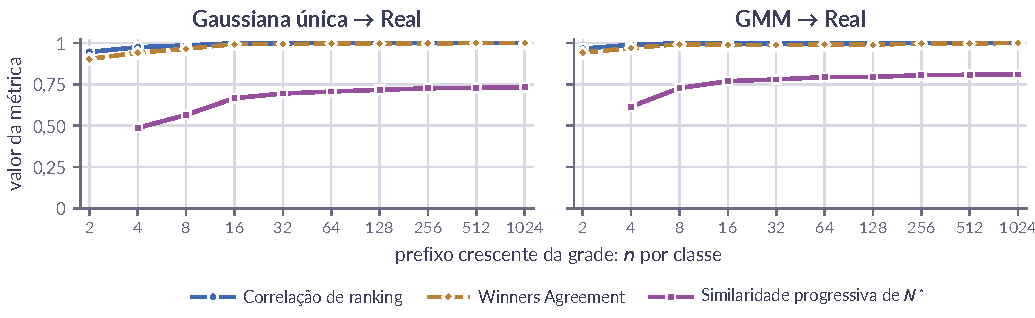
\includegraphics[width=0.94\linewidth]{figures/air_quality_gnb_metricas_progressivas_000006.pdf}\par
  \vspace{0.03cm}
  {\fontsize{7.6}{9.1}\selectfont\color{CoInfoGray}
    Séries persistidas do cenário full-scale 000006; grade até $n=1024$; mesmo teste real fixo.\par}

  \vspace{0.05cm}
  \takeaway{Ranking e relações de vitória são quase integralmente preservados; \Nstar{} permanece mais exigente.}
  \sourcecite{Air Quality: De Vito et al. (2008); cenário full-scale 000006; valores auditados.}

  \speakernotes
    {Aqui acompanhamos a preservação ao longo de toda a grade, não apenas no ponto final. Cada painel corresponde a um braço sintético: à esquerda, classificadores treinados com amostras produzidas por uma Gaussiana única; à direita, com amostras produzidas por um GMM, ambos parametrizados a partir dos dados reais de treinamento. A correlação de ranking e a Winners Agreement ficam próximas de 1 desde os menores prefixos, nos dois braços: a ordenação global por perda média e as decisões par a par são quase integralmente preservadas. A similaridade progressiva de $N^\star$ é claramente menor e evolui de forma diferente: cresce ao longo da grade e estabiliza em torno de 0,73 no braço da Gaussiana única e 0,81 no braço do GMM. Em $n=1024$, ranking e vitórias atingem exatamente 1 nos dois braços. A leitura correta é que a preservação é multidimensional: os dois treinamentos sintéticos reproduzem fortemente a ordenação global e as relações de vencedores, mas reproduzir a posição dos últimos cruzamentos é uma exigência mais estrita, que permanece abaixo de 1.}
    {O terceiro caso separa outra dupla de conceitos: qualidade preditiva absoluta e preservação da estrutura.}
    {Ranking e vitórias quase perfeitos ao longo de toda a grade; $N^\star$ continua revelando diferenças.}
    {1 minuto e 40 segundos.}
    {Não afirmar preservação perfeita de todos os aspectos: a similaridade de $N^\star$ permanece abaixo de 1. Este cenário full-scale estende a grade até 1024; em $n=512$ os valores coincidem com os do cenário full 000005 citado no relatório.}
\end{frame}

% Slide 11 --------------------------------------------------------------------
\begin{frame}{SUPPORT2 — predição $\neq$ estrutura}
  \slidetime{1:40}
  \begin{columns}[T,onlytextwidth]
    \begin{column}{0.48\textwidth}
      \centering
      
\includegraphics[width=\linewidth,height=3.42cm,keepaspectratio]{\figroot/support2_rf_best_losses.pdf}\par
      \vspace{0.06cm}
      {\raggedright\fontsize{7.8}{9.4}\selectfont\color{CoInfoGray}
        Menor perda em $n=512$: Real 0,4555; Gaussiana única 0,4554; GMM 0,4547. Sempre prever a classe majoritária: 0,4687.\par}
    \end{column}
    \begin{column}{0.49\textwidth}
      \centering
      
\includegraphics[width=\linewidth,height=3.42cm,keepaspectratio]{\figroot/support2_rf_metrics.pdf}\par
      \vspace{0.06cm}
      {\raggedright\fontsize{7.8}{9.4}\selectfont\color{CoInfoGray}
        Em $n=512$: GMM melhor em correlação de ranking (0,8665) e \WA{} (0,8429); Gaussiana única melhor em \Nstar{} (0,6799 contra 0,6340).\par}
    \end{column}
  \end{columns}

  \vspace{0.03cm}
  \takeaway{Perda absoluta e preservação da estrutura de cooperação respondem a perguntas diferentes.}
  \sourcecite{SUPPORT: The SUPPORT Principal Investigators (1995); Knaus et al. (1995); cenário full 000008; valores auditados.}

  \speakernotes
    {No SUPPORT2, o Random Forest teve perda mínima próxima de 0,455 nos três braços. O classificador que sempre escolhe a classe majoritária erra 0,4687; portanto, a melhoria absoluta é pequena e o desempenho preditivo é fraco. Ainda assim, a comparação relativa dos 127 subconjuntos mostra que uma parte substancial da estrutura de cooperação foi preservada entre os treinamentos real e sintético. Para classificadores treinados com amostras produzidas pela Gaussiana única, correlação de ranking, Winners Agreement e similaridade de $N^\star$ foram 0,8387, 0,8282 e 0,6799. Com amostras produzidas pelo GMM, 0,8665, 0,8429 e 0,6340. O braço do GMM reproduziu melhor as relações estáticas; o da Gaussiana única, a dinâmica dos últimos cruzamentos. Isso não torna o Random Forest um bom classificador para esse problema: mostra que perda absoluta e preservação estrutural respondem a perguntas diferentes.}
    {Os três estudos de caso permitem uma síntese cuidadosa sobre o que foi e o que não foi demonstrado.}
    {Qualidade preditiva absoluta e preservação da estrutura de cooperação não são equivalentes.}
    {1 minuto e 40 segundos.}
    {Não recomendar Random Forest como melhor classificador e não transformar a elevada preservação estrutural em evidência de boa predição clínica.}
\end{frame}

% Slide 12 --------------------------------------------------------------------
\begin{frame}{Síntese e conclusão}
  \slidetime{1:20}
  \vspace{-0.04cm}
  \begin{columns}[T,onlytextwidth]
    \begin{column}{0.32\textwidth}
      \begin{beamercolorbox}[wd=\linewidth,sep=.12cm,rounded=true]{block body}
        \centering\bfseries\fontsize{10.0}{12.0}\selectfont\color{CoInfoBlue}
        Preservação é\\multidimensional\par\vspace{.07cm}
        \mdseries\fontsize{8.3}{9.9}\selectfont\color{CoInfoInk}
        ranking, vitórias e \Nstar{}\\são complementares
      \end{beamercolorbox}
    \end{column}
    \begin{column}{0.32\textwidth}
      \begin{beamercolorbox}[wd=\linewidth,sep=.12cm,rounded=true]{block body}
        \centering\bfseries\fontsize{10.0}{12.0}\selectfont\color{CoInfoBlue}
        Geometria, perda e\\estrutura são distintas\par\vspace{.07cm}
        \mdseries\fontsize{8.3}{9.9}\selectfont\color{CoInfoInk}
        nenhuma permite inferir\\as outras
      \end{beamercolorbox}
    \end{column}
    \begin{column}{0.32\textwidth}
      \begin{beamercolorbox}[wd=\linewidth,sep=.12cm,rounded=true]{block body}
        \centering\bfseries\fontsize{10.0}{12.0}\selectfont\color{CoInfoBlue}
        Nenhum gerador foi\\universalmente superior\par\vspace{.07cm}
        \mdseries\fontsize{8.3}{9.9}\selectfont\color{CoInfoInk}
        o resultado varia entre\\os cenários avaliados
      \end{beamercolorbox}
    \end{column}
  \end{columns}

  \vspace{0.12cm}
  \takeaway{A preservação da estrutura de cooperação depende da interação entre dataset, classificador, modelo gerador e tamanho amostral.}

  \vspace{0.12cm}
  \begin{beamercolorbox}[wd=\linewidth,sep=.16cm,rounded=true]{block title}
    \centering\bfseries\fontsize{10.2}{12.5}\selectfont
    O resultado principal não é que amostras sintéticas melhorem o classificador: em determinados cenários, o treinamento com amostras sintéticas reproduz a organização cooperativa observada com o treinamento real.
  \end{beamercolorbox}

  \vspace{0.04cm}
  {\centering\fontsize{7.9}{9.4}\selectfont\color{CoInfoGray}
    Extrapolação e decisões de custo não foram validadas; permanecem hipóteses para pesquisa futura.\par}
  \sourcecite{síntese do relatório final do CoInfoSim; cenários full 000002, 000008 e full-scale 000006.}

  \speakernotes
    {A conclusão tem três partes. Primeiro, a preservação estrutural é um perfil multidimensional: correlação de ranking, Winners Agreement e similaridade de $N^\star$ não devem ser fundidas em uma única afirmação. Segundo, semelhança geométrica, desempenho preditivo absoluto e preservação da estrutura de cooperação são propriedades diferentes. Terceiro, nenhum gerador foi universalmente superior nos cenários avaliados: a preservação da estrutura de cooperação depende da interação entre dataset, classificador, modelo gerador e tamanho amostral. Se o treinamento com amostras de um modelo parametrizado a partir dos dados reais reproduzir a estrutura de referência dentro do intervalo observado, esse gerador poderá ser investigado como instrumento para simular regimes amostrais maiores e subsidiar futuras decisões sobre canais. Essa é uma possibilidade de pesquisa, não uma validação já concluída: a grade termina em 512 por classe, 1024 no cenário full-scale, não medimos custos e não demonstramos extrapolação confiável.}
    {Encerrar retomando a tese inicial e, se houver perguntas, usar os slides de apoio para fórmulas, configurações e resultados adicionais.}
    {Em alguns cenários, a estrutura obtida após o treinamento com amostras sintéticas reproduz a organização de referência; isso não prova ganho de acurácia, economia ou extrapolação.}
    {1 minuto e 20 segundos. Duração principal acumulada: 18 minutos e 15 segundos.}
    {Evitar qualquer promessa operacional: custo e extrapolação são hipóteses para validação futura.}
\end{frame}
